\documentclass[11pt]{article}
\usepackage[utf8]{inputenc}
\usepackage[english]{babel}
\usepackage{bilal2vec}
\usepackage{minted}
\title{CS 486 - Assignment 3}
\author{Bilal Khan\\
\href{mailto:bilal2vec@gmail.com}{bilal2vec@gmail.com}}
\date{\today}

\begin{document}

\maketitle
\tableofcontents

\section{1}

\subsection{a}

\begin{minted}{python}
import numpy as np
from collections import defaultdict


def load_data(x_path, y_path):
    x = defaultdict(list)
    y = []

    with open(x_path, 'r') as f:
        for line in f:
            doc_id, word_id = map(int, line.strip().split())
            x[doc_id].append(word_id)

    with open(y_path, 'r') as f:
        for line in f:
            y.append(int(line.strip()))

    return x, y


def train(x, y, n_words):
    n = len(y)

    counts = {1: 0, 2: 0}
    for label in y:
        counts[label] += 1

    prior_probs = {c: count / n for c, count in counts.items()}

    word_counts = {1: np.zeros(n_words + 1), 2: np.zeros(n_words + 1)}

    for doc_id, word_ids in x.items():
        label = y[doc_id - 1]
        for word_id in word_ids:
            word_counts[label][word_id] += 1

    cond_probs = {}
    cond_probs[1] = (word_counts[1] + 1) / (counts[1] + 2)
    cond_probs[2] = (word_counts[2] + 1) / (counts[2] + 2)

    return prior_probs, cond_probs


def pred(x, prior, cond_probs, n_words):
    preds = []

    for doc_id, word_ids in x.items():
        log_posteriors = {}
        for c in [1, 2]:
            log_posterior = np.log(prior[c])

            for word_id in word_ids:
                if word_id <= n_words:
                    log_posterior += np.log(cond_probs[c][word_id])

            for word_id in range(1, n_words + 1):
                if word_id not in word_ids:
                    log_posterior += np.log(1 - cond_probs[c][word_id])

            log_posteriors[c] = log_posterior

        y_hat = max(log_posteriors, key=log_posteriors.get)
        preds.append(y_hat)

    return preds


def accuracy(y_hats, ys):
    n_correct = 0

    for y_hat, y in zip(y_hats, ys):
        if y_hat == y:
            n_correct += 1

    return (n_correct / len(ys)) * 100


if __name__ == "__main__":
    words = []
    n_words = 0
    with open('words.txt', 'r') as f:
        for line in f:
            words.append(line.strip())
            n_words += 1

    x_train, y_train = load_data('trainData.txt', 'trainLabel.txt')

    prior_probs, cond_probs = train(x_train, y_train, n_words)
    y_hats = pred(x_train, prior_probs, cond_probs, n_words)

    train_accuracy = accuracy(y_hats, y_train)
    print(f"trian accuracy {train_accuracy}")

    x_test, y_test = load_data('testData.txt', 'testLabel.txt')

    y_hats = pred(x_test, prior_probs, cond_probs, n_words)

    test_accuracy = accuracy(y_hats, y_test)
    print(f"test accuracy {test_accuracy}")

    log_diffs = []
    for word_id in range(1, n_words + 1):
        log_prob_1 = np.log(cond_probs[1][word_id])
        log_prob_2 = np.log(cond_probs[2][word_id])
        diff = abs(log_prob_1 - log_prob_2)
        log_diffs.append((word_id, diff))

    log_diffs.sort(key=lambda x: x[1], reverse=True)
    top_n_diffs = log_diffs[:10]

    for word_id, diff in top_n_diffs:
        print(f"{word_id} {words[word_id-1]} {diff}")
#trian accuracy 87.86666666666667
#test accuracy 71.26666666666667
#193 christian 3.5835189384561104
#5240 religion 3.5115454388310208
#4662 atheism 3.2958368660043296
#2437 books 3.242592351485517
#1239 christians 3.218875824868201
#4829 library 3.218875824868201
#199 religious 3.091042453358316
#3163 libraries 3.091042453358316
#6898 novel 3.091042453358316
#3522 beliefs 2.9957322735539913
\end{minted}

\subsection{b}

Yes these words seem like they are very distinctive of the subreddits they come from, the log prob diffs are also very high which insprires confidence.

\begin{minted}{text}
christian 3.5835189384561104
religion 3.5115454388310208
atheism 3.2958368660043296
books 3.242592351485517
christians 3.218875824868201
library 3.218875824868201
religious 3.091042453358316
libraries 3.091042453358316
novel 3.091042453358316
beliefs 2.9957322735539913
\end{minted}

\subsection{c}

\begin{minted}{text}
Train accuracy: 87.86666666666667
Test accuracy: 71.26666666666667
\end{minted}  

\subsection{d}

No words in natural language are not independent of each other. The order and context in which you use words mattter, so this assumption is not reasonable.

\subsection{e}

Perform naive bayes on n-grams instead of individual words to capture some contextual information.

\subsection{f}

For maximum likelihood estimation we only need to find parameter values that max the likelihood of the data. For MAP, we would need to define priors for each probability that we want to model (e.g. P(word\_i \| class\_j)).


\section{2}

\subsection{a}

\subsection{b}

\begin{align*}
    mean(mse) &= 0.6172945569875804 \\
    std(mse) &= 0.01777721446341252
\end{align*}

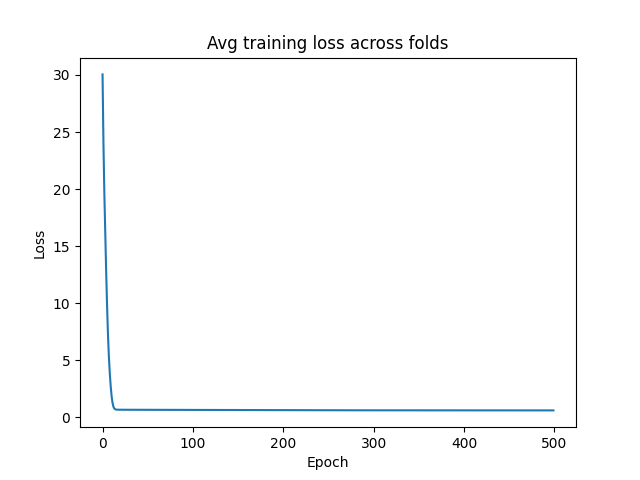
\includegraphics[width=0.5\textwidth]{cross_validation_results.png}

\begin{minted}{python}
import numpy as np
import pandas as pd
import matplotlib.pyplot as plt
from sklearn.model_selection import KFold
from neural_net import NeuralNetwork
from operations import Sigmoid, ReLU, Identity, MeanSquaredError, mean_absolute_error


def load_dataset(csv_path, target_feature):
    dataset = pd.read_csv(csv_path)
    t = np.expand_dims(dataset[target_feature].to_numpy().astype(float), axis=1)
    X = dataset.drop([target_feature], axis=1).to_numpy()
    return X, t


if __name__ == "__main__":
    X, y = load_dataset("data/wine_quality.csv", "quality")
    n_features = X.shape[1]

    folds = KFold(n_splits=5, shuffle=True, random_state=42)

    all_losses = []
    all_maes = []

    fold_idx = 1
    for train_index, val_index in folds.split(X):
        X_train, X_val = X[train_index], X[val_index]
        y_train, y_val = y[train_index], y[val_index]

        net = NeuralNetwork(
            n_features, [32, 32, 16, 1],
            [ReLU(), ReLU(), Sigmoid(), Identity()],
            MeanSquaredError(),
            learning_rate=0.001)

        _, epoch_losses = net.train(X_train, y_train, 500)

        val_mae = net.evaluate(X_val, y_val, mean_absolute_error)

        all_losses.append(epoch_losses)
        all_maes.append(val_mae)
        fold_idx += 1

    avg_losses = np.mean(all_losses, axis=0)
    avg_mae = np.mean(all_maes)
    std_mae = np.std(all_maes)

    print(np.mean(all_losses, axis=1))
    print(avg_mae)
    print(std_mae)

    plt.figure()
    plt.plot(range(500), avg_losses)
    plt.title(f'Avg training loss across folds')
    plt.xlabel('Epoch')
    plt.ylabel('Loss')
    plt.savefig("cross_validation_results.png")
    plt.show()
\end{minted}

\end{document}